\chapter{简单的电现象}

我们生活在电的时代。一座城市,如果完全断了电,简直不堪设想:
工厂停工,电灯不亮,电车不动,电话不通,广播电视停止,自来水供应中断……整个城市几乎陷于停顿。
电,它在工业、农业、交通运输、国防建设、科学研究以及日常生活中用得越来越多,已经成为人类征服自然、改造自然的有力工具。

那么,电是如何产生的呢?为什么它有这么多的应用呢?
要了解这些问题,我们就必须努力学习电的知识。

\section{摩擦起电 两种电荷}\label{sec:7-1}

\begin{wrapfigure}{r}{7cm}
    \centering
    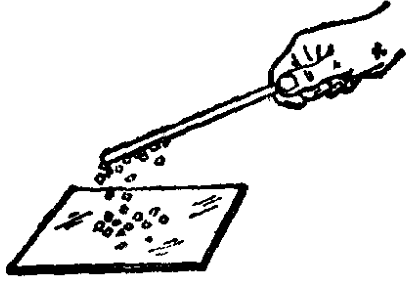
\includegraphics[width=6cm]{../pic/czwl2-ch7-1}
    \caption{丝绸摩擦过的玻璃棒能吸引纸屑}\label{fig:7-1}
\end{wrapfigure}

公元前六世纪的时候,古希腊人发现用毛皮或毛织物摩擦过的琥珀,能够吸引羽毛、头发等轻小物体。
两千多年之后,到十六世纪初,人们进一步知道,不仅毛皮摩擦过的琥珀有这种性质,丝绸摩擦过的玻璃棒,
毛皮摩擦过的硬橡胶棒,绒布摩擦过的硫磺块等,都有这种性质(图 \ref{fig:7-1})。


\CJKunderwave{物体有了吸引轻小物体的性质,我们就说物体带了电,或者说带了电荷}。
用摩擦的方法使物体带电叫做摩擦起电。

摩擦起电的现象在日常生活里也可以看到。
例如,在空气干燥的时候,用塑料梳子梳干净的头发,头发会随着梳子飘起来,
就是因为梳子带了电,吸引头发的缘故。

\begin{figure}[htbp]
    \centering
    \begin{minipage}{7cm}
    \centering
    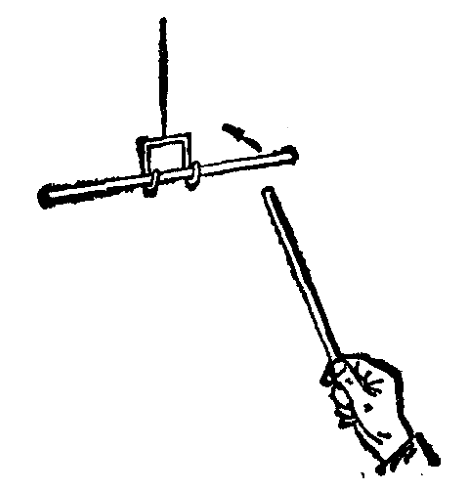
\includegraphics[width=5cm]{../pic/czwl2-ch7-2}
    \caption{}\label{fig:7-2}
    \end{minipage}
    \qquad
    \begin{minipage}{7cm}
    \centering
    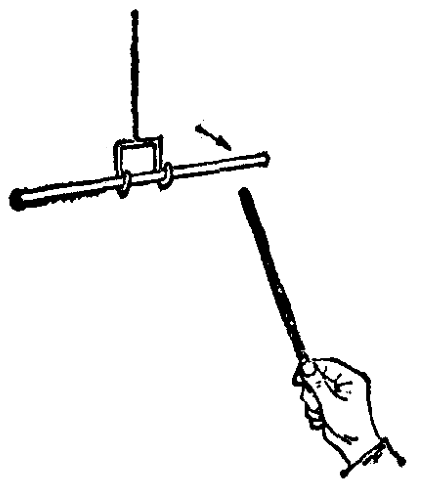
\includegraphics[width=5cm]{../pic/czwl2-ch7-3}
    \caption{}\label{fig:7-3}
    \end{minipage}
\end{figure}

人们研究摩擦起电现象时还发现:用绸子摩擦过的两根玻璃棒互相推斥(图 \ref{fig:7-2}),
用毛皮摩擦过的两根橡胶棒也互相推斥;
但是用绸子摩擦过的玻璃棒跟用毛皮摩擦过的橡胶棒互相吸引(图 \ref{fig:7-3})。
这个现象使人们认识到,用绸子摩擦过的玻璃棒上带的电跟用毛皮摩擦过的橡胶棒上带的电是不同的。
人们用各种各样的物质互相摩擦带电后,发现
凡是跟绸子摩擦过的玻璃棒吸引的,必定跟毛皮摩擦过的橡胶棒推斥;
凡是跟毛皮摩擦过的橡胶棒吸引的,必定跟绸子摩擦过的玻璃棒推斥。
这些事实使人们认识到\CJKunderwave{自然界中只存在两种电荷}。

人们把用绸子摩擦过的玻璃棒带的电荷叫做\textbf{正电荷},
     用毛皮摩擦过的橡胶棒带的电荷叫做\textbf{负电荷}。

\textbf{同种电荷互相推斥,异种电荷互相吸引}。

利用电荷间的相互作用,人们制成了检验物体带不带电的仪器——验电器。
带电体接触验电器的金属球的候(图 \ref{fig:7-4}),就有一部分电荷转移到验电器的两片金属箔上,
这两片金属箔由于带同种电荷互相推斥而张开。
我们从金属箔的张开可以断定跟金属球接触的物体是带电的。

\begin{figure}[htbp]
    \centering
    \begin{minipage}{7cm}
    \centering
    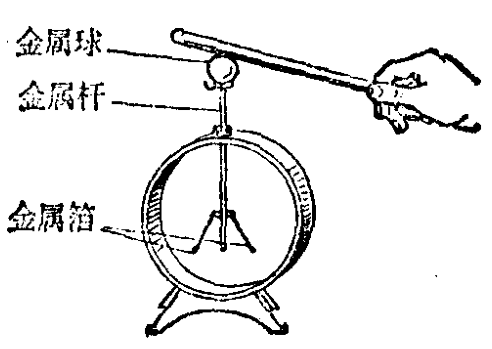
\includegraphics[width=6cm]{../pic/czwl2-ch7-4}
    \caption{}\label{fig:7-4}
    \end{minipage}
    \qquad
    \begin{minipage}{7cm}
    \centering
    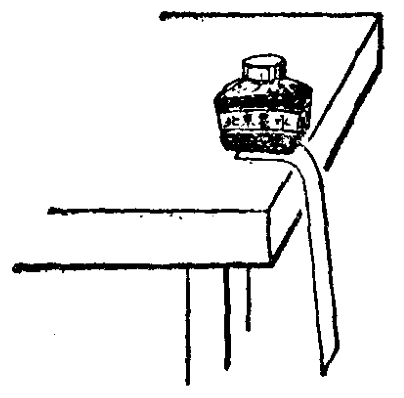
\includegraphics[width=5cm]{../pic/czwl2-ch7-5}
    \caption{}\label{fig:7-5}
    \end{minipage}
\end{figure}

\section*{小实验}

剪一些碎纸屑。从塑料薄膜上剪下 20 厘米长、2 厘米宽的两条。

把一条塑料薄膜铺在桌面上,用手帕(或丝绸)在薄膜上摩擦几下,然后利用纸屑检查薄膜条是不是带了电。

把带了电的薄膜条上端压在桌边上(图 \ref{fig:7-5})。

用手帕摩擦另一条塑料薄膜,然后把这条塑料薄膜拿近压在桌边的那一条,看到了什么现象?为什么?

把手帕拿近压在桌边的薄膜条,看到了什么现象?为什么?


\section{摩擦起电的原因}\label{sec:7-2}

我们从化学课里已经知道,有些物质是直接由原子构成的,有些物质是由分子构成的,而分子也是由原子构成的。
原子的中心是由带正电的质子和不带电的中子组成的原子核,核的周围是高速运动的带负电的电子。
在通常情况下,原子核带的正电跟核外电子总共带的负电数量相等,整个原子是中性的。
图 \ref{fig:7-6} 是氢、氦、锂的原子结构的模型。

\begin{figure}[htbp]
    \centering
    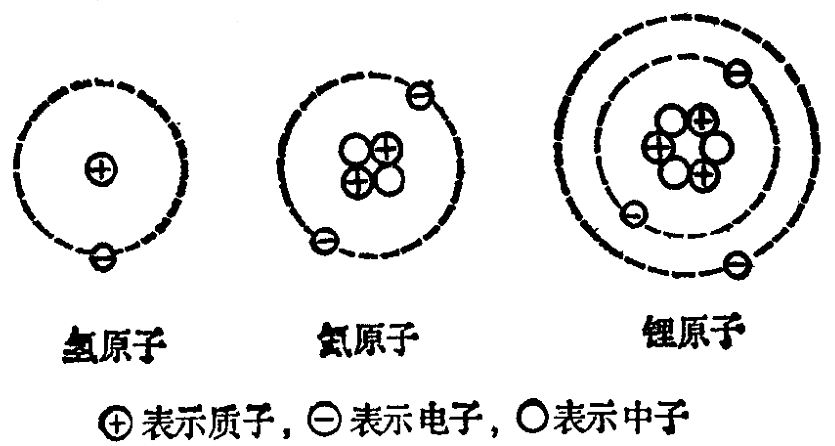
\includegraphics[width=0.6\textwidth]{../pic/czwl2-ch7-6}
    \caption{氢、氦、锂的原子结构模型}\label{fig:7-6}
\end{figure}

本来是中性的原子,当它失去一个或几个电子的时候,它的电子总共带的负电数量比原子核的正电少,它就显示出带正电;我们称它为正离子。
相反,本来是中性的原子,当它跟多余的电子结合在一起的时候,它就显示出带负电;我们称它为负离子。

在通常情况下,由于原子是中性的,因而物体也呈中性。
那么,当两个物体相互摩擦的时候,为什么物体能带电呢?
原来,不同物质的原子核束缚电子的本领不同。
当两个物体相互摩擦的时候,哪个物体的原子核束缚电子的本领较弱,它的一些电子就会转移到另一个物体上。
失去电子的物体因缺少电子而带正电,得到电子的物体则因有了多余电子而带等量的负电。
例如玻璃跟绸子摩擦,玻璃的一些电子转移到绸子上,玻璃因失去电子而带正电,绸子因得到电子而带等量的负电。
橡胶跟毛皮摩擦,毛皮的一些电子转移到橡胶上,橡胶带负电,毛皮带等量的正电。

可见,摩擦起电并不是创造了电,只是电子从一个物体转移到另一个物体。

我们如果让两个带等量的异种电荷的物体互相接触,带负电的物体上多余的电子转移到带正电的物体上,
那么,这两个物体都没有多余的电子,也不缺少电子,都恢复成不带电的状态。
这种现象叫做正、负电荷的中和。



\section*{阅读材料:人类对摩擦起电的认识}

摩擦起电的现象虽然发现很早,但是在长达两千多年的时间里,只停留在观察琥珀的摩檫起电上。
第一个认真研究电现象的是英国医生吉尔伯特(1540 ~ 1603),他想搞清楚琥珀为什么会有那种神奇的吸引力。
1600 年,他发现金刚石、水晶、硫磺、火漆和玻璃等物质,在用呢绒、毛皮或丝绸摩擦过后,象琥珀那样有神奇的吸引力。
这使他领悟到这种现象并不是琥珀特有的,于是他想可能一切物质中都蕴藏着一种看不见的流体,
当受到摩擦的时候从物质中被挤出来,他把这种看不见的特殊流体叫做“电"。这是对摩擦起电现象最早的猜想。

1734 年,法国化学家杜菲发现电有两种,同种电相异斥,异种电相吸。
他把这两种电分别叫“玻璃电”和“琥珀电”。
当带“玻璃电”的物体和带“琥珀电”的物体互相接触的时候,电的性质会减弱甚至消失,
象正、负数能互相抵消一样,所以美国学者富兰克林(1706~1790)把它们叫“正电”和“负电”。
1747 年富兰克林还提出一种假说,被称为“单流休说”,用来解释摩擦起电。
这种假说认为:在一切物质中都存在着一种正的“电流体”,物林中的“电流体”
比正常状态的时候多,物体就带正电,
比正常状态的时候少,物体就带负电;
两个物体互相摩擦,“电流体”从一个物体流入另一个物体,所以一个带正电,一个带负电。

1759 年,英国物理学家塞麦发展了杜菲的看法,提出了新的“双流体说”,认为一切物质中都存在两种“电流体”,
一种是正的,一种是负的;正常状态下的物体中,这两种流体的量相等,它们的作用互相抵消了。
当两个物体互相摩擦的时候,就会有流体的转移,结果,
  一个物体中的正流体超过平衡量,显示带正电,
另一个物体中的负流体超过平衡量,显示带负电。

单流体说的支持者和双流体说的支持者有过长期的争论,但是直到十九世纪末还没有令人信服的实验表明哪一个正确。
二十世纪初人类认识了原子的结构以后才知道,这两种假说都有正确的成份。
事实上,物体中既有正电荷,又有负电荷,双流体说在这一点上是正确的;
但是在摩擦起电时,只是带负电荷的电子从一个物体流入另一物体,在只是有一种电荷能够流动这一点上,单流体说是正确的。


\lianxi

\begin{wrapfigure}{r}{5cm}
    \centering
    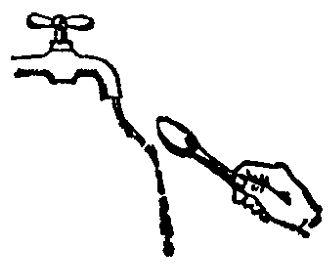
\includegraphics[width=4cm]{../pic/czwl2-ch7-7}
    \caption{}\label{fig:7-7}
\end{wrapfigure}

(1) 用什么方法可以检验出经过摩擦的物体是否带上了电?

(2) 当验电器上的金属球跟带正电的物体接触时,金属球也带上了正电。你能够解释这种现象吗?

(3) 当验电器上的金属球跟带负电的物体接触时,金属球也带上了负电。你能够解释这种现象吗?

(4) 用带电体去靠近吊在细线上的通草球时,由于带电体能够吸引轻小物体,所以通草球会被带电体吸引过来。
但接触后立即就离开了。这是为什么?

(5) 做下面的实验:把水龙头稍微拧开一点,让它流出很细的水流。拿一把塑料勺(或塑料尺等)在毛织品上摩擦几下,
然后把它靠近水流,可以看到水流被勺子吸引而弯曲了(图 \ref{fig:7-7})。
如果没有水龙头,你能不能想出什么办法得到一股细的水流来做这个实验?


\section{导体和绝缘体}\label{sec:7-3}

电线里面的芯都是金属丝,在金属丝的外面还要包上一层橡皮或者塑料,这是为什么呢?
为了说明这个问题,我们来做个实验。

\begin{figure}[htbp]
    \centering
    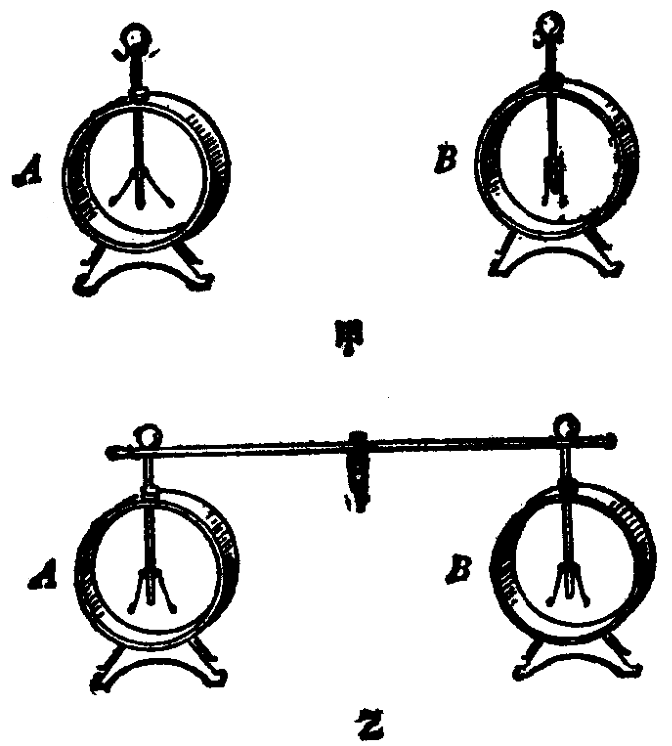
\includegraphics[width=0.6\textwidth]{../pic/czwl2-ch7-8}
    \caption{}\label{fig:7-8}
\end{figure}

取两个相同的验电器 $A$、$B$,使 $A$ 带电,$B$ 不带电(图 \ref{fig:7-8} 甲)。
拿一根带橡胶柄的金属棒,把这两个验电器连接起来,可以看到,
$B$ 的金属箔张开了,同时 $A$ 的金属箔张开的角度减小了(图 \ref{fig:7-8} 乙)。
这表示 $A$ 上的一部分电荷通过金属棒传到 $B$ 上去了。
如果不用金属棒,而用玻璃棒或橡胶棒来连接 $A$ 和 $B$,$B$ 的金属箔就不张开。
这表示 $A$ 上的电荷不能够通过玻璃棒或橡胶棒传到 $B$ 上去。

上面的实验表明,有的物体容易导电,有的物体不容易导电。

容易导电的物体叫做\textbf{导体}。金属、人体、大地以及各种酸、碱、盐的水溶液都是导体。

不容易导电的物体叫做\textbf{绝缘体}。橡胶、塑料、玻璃、陶瓷、油、空气都是好的绝缘体。

为什么导体能够导电,绝缘体不能够导电呢?
原来,导体中有能够自由移动的电荷,因此在导体里电荷能够从一个地方传到别的地方。
绝缘体中的电荷几乎都被束缚在原子或分子的范围内,不能自由移动,因此在绝缘体里电荷不能从一个地方传到别的地方。
金属是最重要的导体,在金属里能够自由移动的电荷就是电子,这种能自由移动的电子叫做\textbf{自由电子}。
在酸、碱、盐的水溶液里,能够自由移动的电荷是正离子和负离子。

好的导体和好的绝缘体都是重要的电工材料,在技术上应用很广。
电线芯用金属来做,是因为金属是导体,能够导电;
外面包上一层橡皮或者塑料,是因为这些材料是绝缘体,能防止漏电或触电。
许多电学仪器,有的部分需要用导体来做,有的部分又需要用绝缘体来做。

导体和绝缘体并没有绝对的界线,在通常情况下是很好的绝缘体,当条件改变时也可能变成导体。
例如,如果用一根干木棒把图 \ref{fig:7-8} 中的两个验电器连起来,会看到干木棒不导电。
把这根木棒弄湿,会看到湿木棒导电了。这表明,绝缘体潮湿了会导电。
因此,电器的绝缘部分要保持干燥,以免漏电和发生触电事故。

除了导体和绝缘体,还有一类物体,它们的导电能力在导体和绝缘体之间,叫做半导体。
由于半导体有许多独特而有用的性质,因而在电子技术和无线电技术中有着广泛的应用。


\lianxi

\begin{wrapfigure}[10]{r}{7cm}
    \centering
    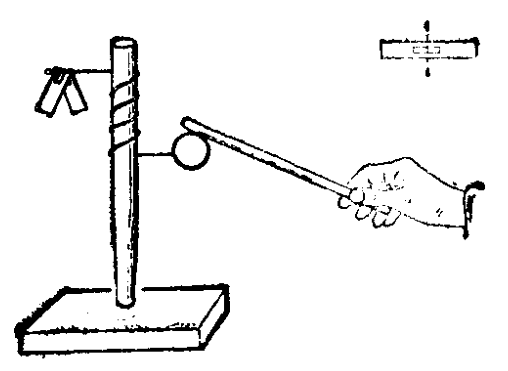
\includegraphics[width=6cm]{../pic/czwl2-ch7-9}
    \caption{自制的简单验电器}\label{fig:7-9}
\end{wrapfigure}

(1) 为什么用摩擦的方法可以使拿在手中的胶木棒带电,却不能使拿在手中的金属棒带电?
怎样才能使拿在手中的金属棒带电?

(2) 电工修电路的时候,使用有木柄或者柄上套着橡胶套的工具,并且常常站在干燥的木凳上,为什么?

(3) 观察一下验电器,看看它的哪些部分是导体,哪些部分是绝缘体?

(4) 在图 \ref{fig:7-4} 中,为什么带电体接触验电器金属棒上端的金属球,金属棒下端的两条金属箔就会张开?

(5) 照图 \ref{fig:7-9} 那样,把塑料笔杆插在座子上(座子可以用橡皮泥或泥土来做),在笔杆上缠一段金属丝。
金属丝的左端挂一条对折的金属箔(可以用包纸烟的金属箔照图 \ref{fig:7-9} 右上角画的那样剪好沿虚线对折),
金属丝的右端绕成环状,这样就做成了一个简单的验电器。
当带电体接触右边的金属环时,左边的金属箔就张开,为什么?
自己做一个简单的验电器,并且用它检验跟头发摩擦过的塑料梳子带不带电。


\section{电流}\label{sec:7-4}

在图 \ref{fig:7-8} 的实验里,用金属棒把带电的验电器 $A$ 和不带电的验电器 $B$ 连接起来,
就有一部分电荷从验电器 $A$ 通过金属棒传到验电器 $B$ 上去。这表示在金属棒中发生了电荷的移动。

\textbf{电荷的定向移动形成电流}。

重作图 \ref{fig:7-8} 的实验,会看到不带电的验电器 $B$ 的金属箔张开到一定的角度,就不再张大了,
表明电荷不再通过金属棒往验电器 $B$ 上移动了,金属棒中不再有电流了。
这种情况下金属棒中的电流只存在一瞬间。

我们通常需要的是持续的电流。
例如,我们利用电来照明或者利用电来使电动机转动,都需要电流长时间地持续存在。
那么,怎样才能得到持续的电流呢?

接下手电筒的接钮,手电筒的小灯泡就发光。
小灯泡持续发光,表明我们得到的电流是持续的。
这个电流能持续存在,是因为电筒里有干电池不断供电的缘故。
如果电筒里没有干电池,无论怎样按按钮,灯都不亮。

闭合电动机的开关,电动机就转个不停,表明电流是持续的。
这个电流能持续存在,是因为发电厂的发电机不断供电的缘故。
如果发电机停止运行,即使闭合了电动机的开关,电动机也不旋转。

象干电池、发电机这些能够持续供电的装置,叫做电源。
\CJKunderwave{要得到持续的电流必须有电源}。

电流的方向是怎样的呢?导体中的电流是自由电荷定向移动形成的。
定向移动的既可能是正电荷(如正离子),也可能是负电荷(如负离子或电子),还可能是正负电荷同时向相反方向移动。
在科学上规定电流方向的时候,人们还不了解各种导体的导电情况,把\textbf{正电荷定向移动的方向规定为电流的方向}。

金属导体中形成电流的是带负电的自由电子的定向移动。
根据电流方向的规定知道,\CJKunderwave{金属导体中的电流方向跟自由电子的实际移动方向相反}。
但是,正负电荷向相反方向移动所产生的效果相同,
因此,金属导体中的电流方向虽然跟自由电子的实际移动方向相反,却不影响我们研究有关电流的问题。


\section{电池}\label{sec:7-5}

\begin{wrapfigure}[12]{r}{7cm}
    \centering
    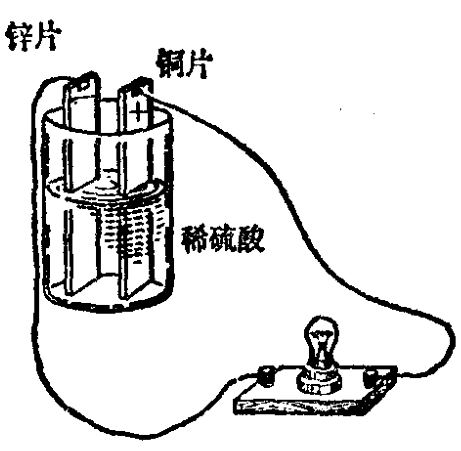
\includegraphics[width=6cm]{../pic/czwl2-ch7-10}
    \caption{用伏打电池给小灯泡供电}\label{fig:7-10}
\end{wrapfigure}

电池是日常生活中和实验室里常用的电源。
最初的电池是十九世纪初意大利物理学家伏打发明的,叫伏打电池。
把一块铜片和一块锌片,浸在稀硫酸溶液里,就做成了一个伏打电池,
它可以向小灯泡供电,使小灯泡发光(图 \ref{fig:7-10})。
在伏打电池里,由于发生了化学变化,在铜片上聚集了正电荷,在锌片上聚集了负电荷。
铜片和锌片叫做伏打电池的电极。
聚集正电荷的铜片叫\textbf{正极},
聚集负电荷的锌片叫\textbf{负极}。
用导线把小灯泡连接到电池的两极间时,电流从电池的正极流出,经过导线和小灯泡,流回电池的负极。
所以,\CJKunderwave{导线中电流的方向是从电池的正极流向负极}。

用伏打电池作电源,小灯泡很快就暗下来,表明通过灯丝的电流迅速地减弱。
所以这种电池实用价值不大,现在最常用的电池是干电池。

干电池的外壳是一个锌筒,\CJKunderwave{锌筒是干电池的负极},也是干电池的容器,里面装着化学药品。
锌筒中央的\CJKunderwave{碳棒是干电池的正极}(图 \ref{fig:7-11})。

\begin{figure}[htbp]
    \centering
    \begin{minipage}{7cm}
    \centering
    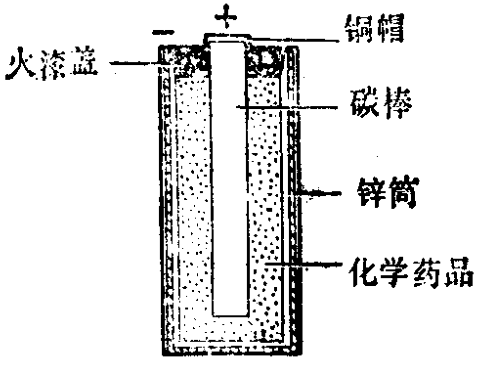
\includegraphics[width=6cm]{../pic/czwl2-ch7-11}
    \caption{干电池剖面图}\label{fig:7-11}
    \end{minipage}
    \qquad
    \begin{minipage}{7cm}
    \centering
    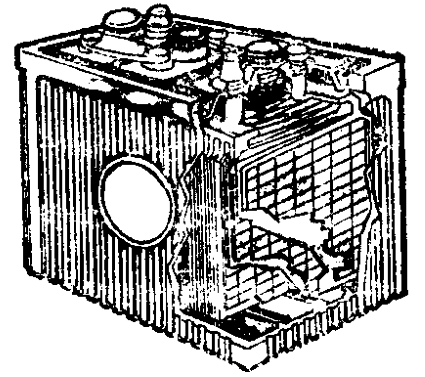
\includegraphics[width=6cm]{../pic/czwl2-ch7-12}
    \caption{铅蓄电池}\label{fig:7-12}
    \end{minipage}
\end{figure}


干电池连续使用长了电流会减弱,所以干电池适合于断续的工作,
半导体收音机、手电筒等等常用干电池作电源。

干电池用过相当长的时间以后,就不能再用了,必须换新的。
这类电池叫一次电池,也叫原电池。
还有一类电池叫蓄电池,可以多次充电重复使用。

图 \ref{fig:7-12} 是常用的铅蓄电池。这种电池是把许多块铅板放在稀硫酸里做成的。
铅板分为两组,一组是正极,一组是负极,它们的接线柱上分别有 “$+$” 、“$-$” 的标记。

为了使蓄电池能向外供电,需要先给它充电。
充电的时候,要把蓄电池的正、负极分别接到另一个电源的正、负极上,电流通过蓄电池,
使蓄电池内部发生化学变化,电能转化为化学能,储蓄在蓄电池里。
蓄电池向外供电叫做放电,放电的时候,它储蓄的化学能又转化为电能。

蓄电池的应用很广。汽油机的点火,汽车、火车、飞机的照明,等等,都要用到蓄电池。
做物理实验的时候也常常用蓄电池作为电源。

使用蓄电池的时候,\CJKunderwave{绝对不允许用导线直接把两极连接起来}(其他电源也不允许这样做),
因为那样放电电流太大,会损坏蓄电池。蓄电池用过一段时间以后,需要及时给它充电,不然也会损坏。

上面讲到的几种电池,都是利用化学变化来供电的。
从能量转化的观点来看,它们的作用都是把化学能转化成电能。这样的电池又叫做化学电池。


\section*{阅读材料:新型电池}

干电池、铅蓄电池的应用已经有一百多年的历史,它们的性能虽然不断提高,
但是满足不了科学技术各方面飞速发展的需要。因此,近年来新型电池不断出现。

氧化银电池(也叫银锌电池)是一种重量轻而容量\footnotemark 大的新电池,大量用在电子手表、导弹和人造卫星上。
它的负极是锌,正极是氧化银。图 \ref{fig:7-13} 是用于电子手表里的钮扣式微型氧化银电池,可以连续使用一年。
\footnotetext{电池放电电荷的总量叫做电池的容量。}

\begin{figure}[htbp]
    \centering
    \begin{minipage}{8cm}
    \centering
    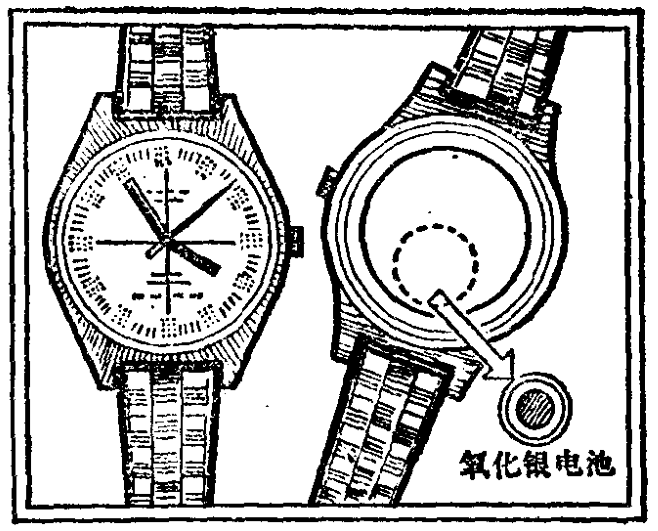
\includegraphics[width=7cm]{../pic/czwl2-ch7-13}
    \caption{电子手表里的微型氧化银电池}\label{fig:7-13}
    \end{minipage}
    \qquad
    \begin{minipage}{6cm}
    \centering
    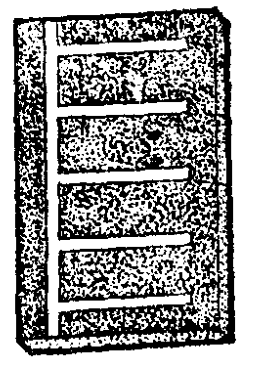
\includegraphics[width=3cm]{../pic/czwl2-ch7-14}
    \caption{硅光电池}\label{fig:7-14}
    \end{minipage}
\end{figure}


锂电池是一种正处于试用阶段尚未大量生产的新型电池,它的负极是锂做的。
这种电池的突出优点是使用寿命长,能在较大的温度范围内工作。

还有一些不属于化学电池的新型电池,例如硅光电池(图 \ref{fig:7-14})。
硅光电池是用硅做成的、把光能转化为电能的电池。
这种电池性能稳定,寿命很长,但目前成本高、价格贵,主要用在人地球卫星上,%(\hyperref[fig:pic4]{彩图4}),
作为卫星携带的实验仪器、通讯设备的电源。
现在,把原子能直接转化为电能的原子电池,也在开始研究试制了。


\section{电流的效应}\label{sec:7-6}

导体中有没有电流,看不见也听不着,那么怎么才能知道呢?这个似乎不好解决的问题其实是很容易解决的。
原来,导体中有电流的时候,会发生一些特有的现象,根据这些现象就可以判定电流的存在。
我们把导体中有电流的时候发生的现象,叫做电流的效应。

电灯泡里的灯丝通过电流发光的时候,用手摸摸灯泡,可以觉得它比不发光的时候热。
从实验知道,一切导体,有电流通过的时候,都要发热。
\CJKunderwave{任何导体中有电流的时候,导体都要发热,这种现象叫做电流的热效应}。
电炉、电烙铁都是利用电流的热效应来工作的。

把两根碳棒立在盛着硫酸铜溶液的玻璃杯里,用导线把两根碳棒分别跟电池的两极连接起来(图 \ref{fig:7-15}),
在硫酸溶液中就有了电流,过几分钟后,跟负极相连的碳棒上出现一层红色的铜,这层铜是从硫酸铜溶液里分解出来的。
可见,\CJKunderwave{在导电的溶液里有电流的时候,溶液里要发生化学变化,这种现象叫做电流的化学效应}。
工业上利用电流的化学效应来提炼铝、铜等金属,以及在容易生锈的金属物品上镀一层防锈的金属。

\begin{figure}[htbp]
    \centering
    \begin{minipage}{7cm}
    \centering
    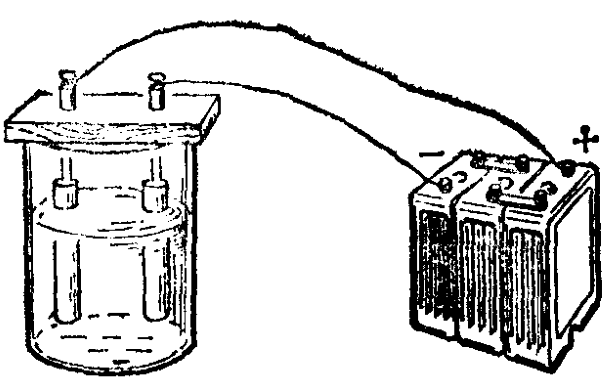
\includegraphics[width=6cm]{../pic/czwl2-ch7-15}
    \caption{}\label{fig:7-15}
    \end{minipage}
    \qquad
    \begin{minipage}{7cm}
    \centering
    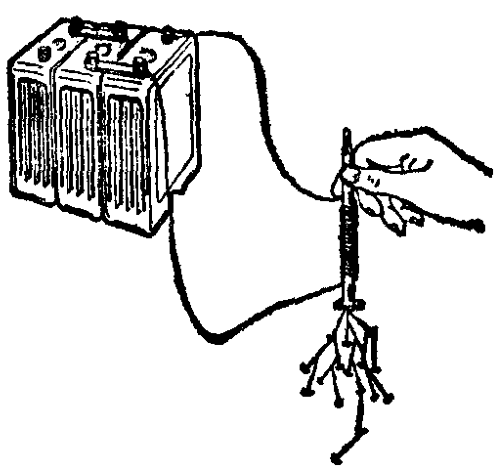
\includegraphics[width=6cm]{../pic/czwl2-ch7-16}
    \caption{}\label{fig:7-16}
    \end{minipage}
\end{figure}

在图 \ref{fig:7-16} 所示的实验中,把绝缘导线缠在一根铁钉上,当有电流通过时,铁钉能够吸引轻小的铁质东西如大头针、铁屑等,
表明铁钉变成了磁铁。电流一停止流通,被吸的东西就掉下来。
可见,\CJKunderwave{当导线中有电流的时候,在导线周围就产生跟磁铁相同的作用,这种现象叫做电流的磁效应}。

电流的各种效应,不但能使我们觉察电流的存在,而且使电流在许多方面获得了广泛的应用。
我们在这一节里只是初步提到某些应用,在后面还要继续学习。


\lianxi

(1) 在图 \ref{fig:7-17} 里,导线(或灯泡)中的电流方向是从锌筒到碳棒,还是从碳棒到锌筒?自由电子定向移动的方向呢?

\begin{figure}[htbp]
    \centering
    \begin{minipage}{7cm}
    \centering
    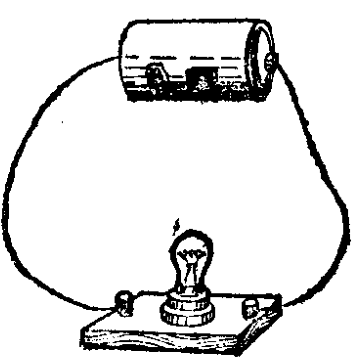
\includegraphics[width=4cm]{../pic/czwl2-ch7-17}
    \caption{}\label{fig:7-17}
    \end{minipage}
    \qquad
    \begin{minipage}{7cm}
    \centering
    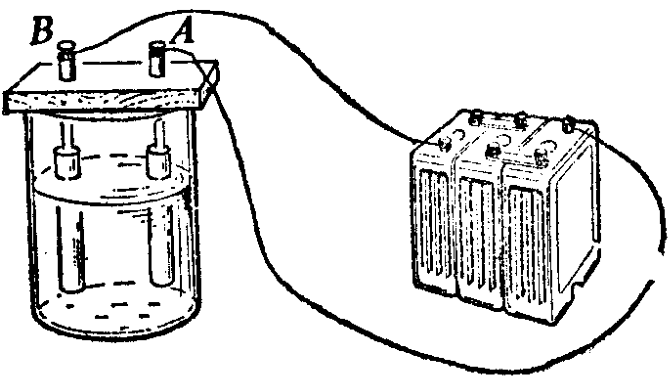
\includegraphics[width=6cm]{../pic/czwl2-ch7-18}
    \caption{}\label{fig:7-18}
    \end{minipage}
\end{figure}

(2) 在图 \ref{fig:7-18} 所示的装置里,碳棒 $A$、$B$ 立在硫酸铜溶液里,通电以后在碳棒 $A$ 上出现了一层红色的铜。
能不能根据这个现象确定电源的正、负极?在图中标出电流的方向。

\begin{figure}[htbp]
    \centering
    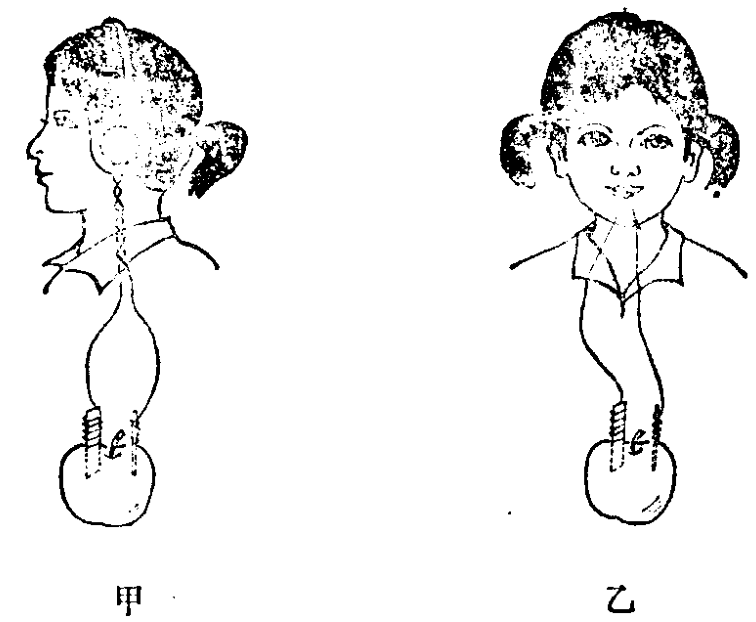
\includegraphics[width=0.6\textwidth]{../pic/czwl2-ch7-19}
    \caption{}\label{fig:7-19}
\end{figure}

(3) 做一个水果电池:找一根 5 厘米长的铜片或粗铜丝(也可以用绞在一起的几根细铜丝来代替),
再从废干电池上剪一条 2 毫米宽的锌皮,刮净,把铜丝和锌皮插入苹果或别的水果(也可以用番茄或土豆)里,
就做成了一个水果电池。将耳机线一根的末端接到一个电极上,当另一根的末端跟另一个电极断续接触时(图 \ref{fig:7-19} 甲),
从耳机里能听到电流引起的喀拉喀拉的声音。
也可以取两根导线,把它们的一端分别接到水果电池的两极,另一端和舌头断续接触(图 \ref{fig:7-19} 乙),
注意两根导线不要碰着,这时舌头上有什么异样的感觉?


\section{电路}\label{sec:7-7}

\begin{wrapfigure}[8]{r}{7cm}
    \centering
    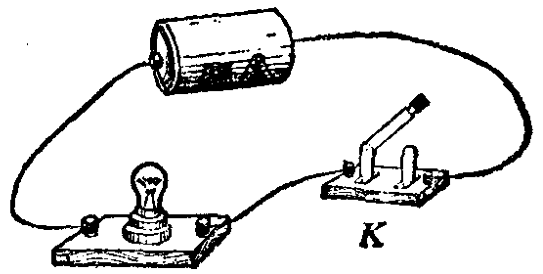
\includegraphics[width=6cm]{../pic/czwl2-ch7-20}
    \caption{}\label{fig:7-20}
\end{wrapfigure}

\xiaobiaoti{电路和电路图}
电灯、电铃、电炉和电动机等利用电流来工作的设备,都叫做用电器。
为了把电流送给用电器,必须用导线把电源和用电器连接起来。
为了随时能够把用电器跟电源连通或者切断,还必须安装开关——电键。

由电源、用电器以及导线、电键等元件组成的电流路径,叫做\textbf{电路}。
图 \ref{fig:7-20} 就是一个简单的电路。
在这个电路中,干电池是电源,小灯泡是用电器,连接电路用的电线就是导钱,$K$ 是电键。

要使电路中有电流,电路必须是处处连通的,处处连通的电路叫做通路。
如果电路中某处断开了,电路不再闭合,电路中就没有电流了。断开的电路叫做断路。

\begin{figure}[htbp]
    \centering
    \begin{minipage}{11cm}
    \centering
    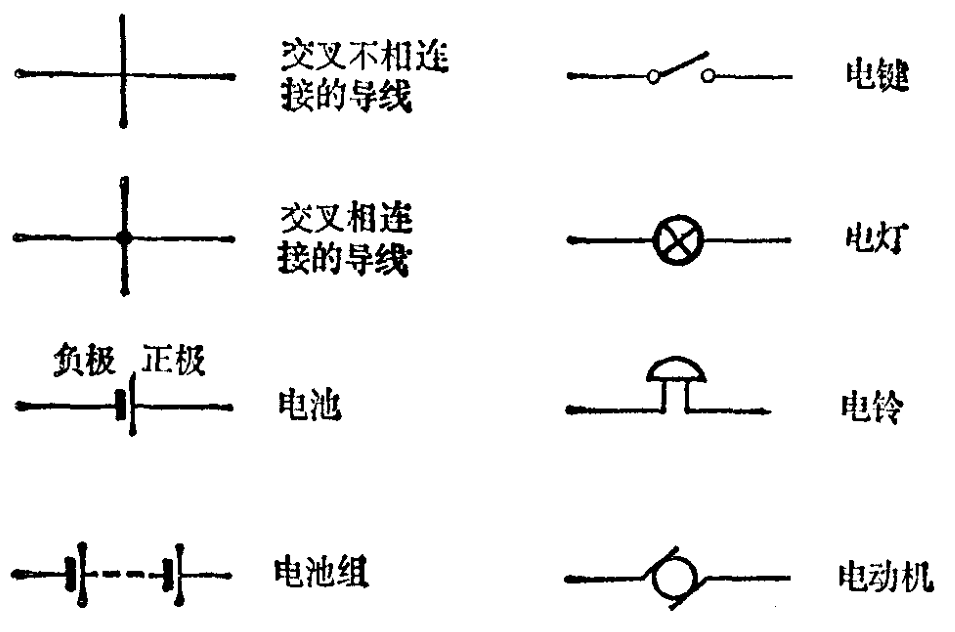
\includegraphics[width=10cm]{../pic/czwl2-ch7-21}
    \caption{几种电路元件的符号}\label{fig:7-21}
    \end{minipage}
    \qquad
    \begin{minipage}{5cm}
    \centering
    \vspace{4cm}
    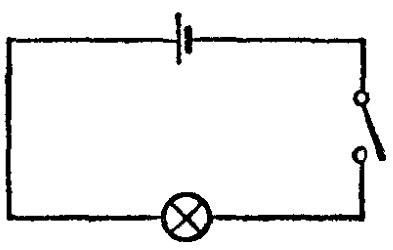
\includegraphics[width=4cm]{../pic/czwl2-ch7-22}
    \caption{}\label{fig:7-22}
    \end{minipage}
\end{figure}


在设计、安装、修理各种实际电路的时候,常常需要画出表示电路连接情况的图。
为了简便,通常不画实物图,而用国家统一规定的符号来代表电路中的各种元件(图 \ref{fig:7-21})。
这种用规定的符号表示电路连接情况的图,叫做电路图。
图 \ref{fig:7-22} 就是图 \ref{fig:7-20} 的电路图。


\xiaobiaoti{串联和并联}
在一个电路里连接的用电器往往不只一个。
如果要在一个电路里连接两盏电灯,有几种连接方法呢?

\begin{figure}[htbp]
    \centering
    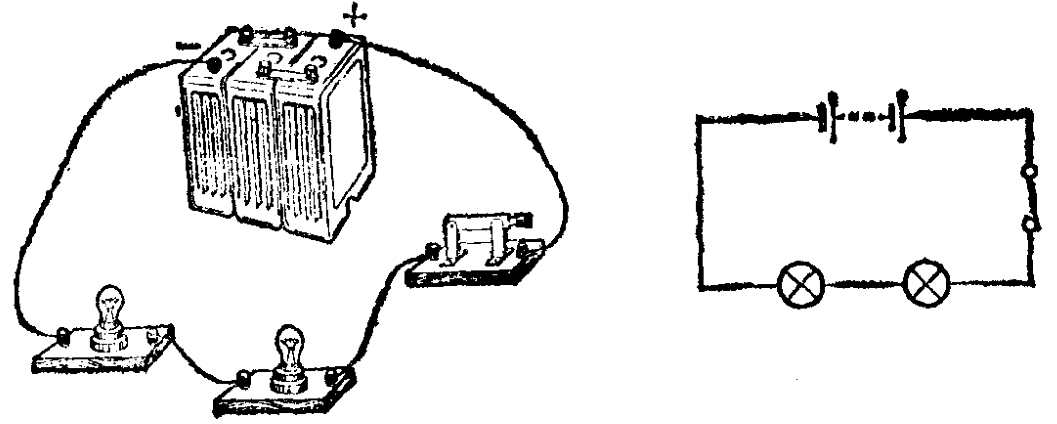
\includegraphics[width=0.7\textwidth]{../pic/czwl2-ch7-23}
    \caption{串联电路}\label{fig:7-23}
\end{figure}

我们可以接照图 \ref{fig:7-23} 那样,把两电灯顺次连接在电路里。
把电路元件逐个顺次连接起来的方法叫做\textbf{串联}。
从图 \ref{fig:7-23} 可以看出,在串联电路里,通过一盏灯的电流也要通过另一盏灯。
如果熄灭一盏电灯(把灯泡从灯座上去掉),电路就被断开,另一盏灯也就不亮了。


我们还可以照图 \ref{fig:7-24} 那样,把两盏电灯并列接在电路的两点间。
把电路元件并列接在电路两点间的连接方法叫做\textbf{并联}。
从图 \ref{fig:7-24} 可以看出,在并联电路里,干路中的电流在分支处分成两部分,
一部分电流通过一盏电灯,另一部分电流通过另一盏电灯。
断开一条支路,这条支路中的电灯就熄灭,
但是另一条支路中的电灯仍旧继续发光,因为它与干路构成的整个电路仍旧是通路。

\begin{figure}[htbp]
    \centering
    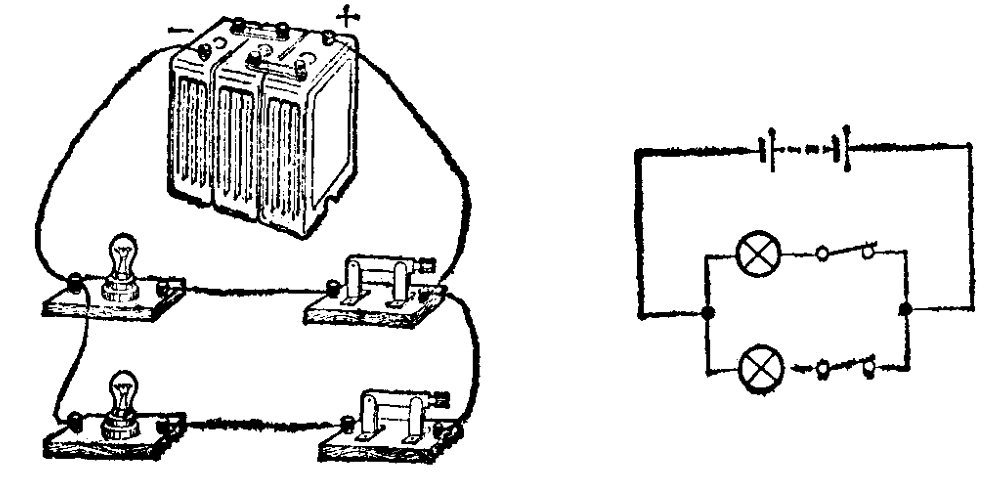
\includegraphics[width=0.7\textwidth]{../pic/czwl2-ch7-24}
    \caption{并联电路}\label{fig:7-24}
\end{figure}


串联和并联是两种最基本的电路连接方法,在实验室里和生产技术中都常常用到。


\section{实验:组成串联电路和并联电路}\label{sec:7-8}

在这个实验里,我们要自己动手连接简单的电路,学习和掌握串联、并联这两种最基本的电路连接方法。

我们要连接的是图 \ref{fig:7-25} 和图 \ref{fig:7-26} 所示的电路。
需要哪些器材(包括名称和数量),自己可以根据图列出清单,再按清单检查实验桌上的器材是否够用。

(1) 组成串联电路

接照图 \ref{fig:7-25} 组成串联电路。
连接电路的时候应该按照一定的顺序,这个顺序可以自己定,
例如可以顺着电流的方向从电池组的正极开始接线,再依次接好电键 $K$、灯 $L_1$、灯 $L_2$,最后连接电池组的负极,
也可以逆着电流的方向从电池组负极开始接线,依次接好 $L_2$、$L_1$、$K$,最后连接电池组正极。
必须注意,在连接电路的过程中,电键应该是断开的。

电路接好后,先闭合再断开电键,观察串联电路里的电键是同时控制两个灯泡,还是只控制其中一个。

把电键 $K$ 改接到 $L_1$ 和 $L_2$ 之间,再改接到 $L_2$ 和电池组负极之间,
每一次都闭合、断开电键,观察电键的控制作用是否改变了。

分别画出上面三次实验的电路图,在图旁记下观察结果。
根据上面的实验回答;串联电路里的电键是同时控制两个灯泡,还是只控制其中一个?
在串联电路里,电键的位置改变了,它的作用有没有改变?

\begin{figure}[htbp]
    \centering
    \begin{minipage}{7cm}
    \centering
    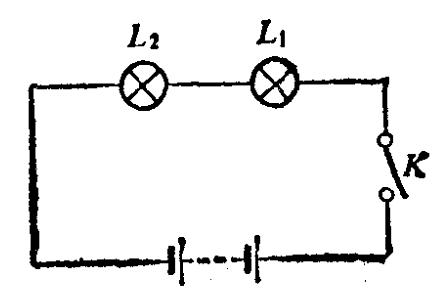
\includegraphics[width=6cm]{../pic/czwl2-ch7-25}
    \caption{}\label{fig:7-25}
    \end{minipage}
    \qquad
    \begin{minipage}{7cm}
    \centering
    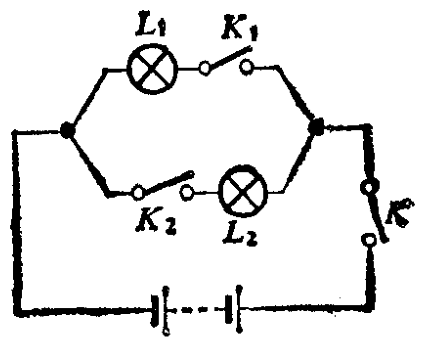
\includegraphics[width=6cm]{../pic/czwl2-ch7-26}
    \caption{}\label{fig:7-26}
    \end{minipage}
\end{figure}


(2) 组成并联电路

照图 \ref{fig:7-26} 组成并联电路。把三个电键都闭合,然后进行下述观察:

断开、闭合干路电键 $K$,观察它控制哪个灯泡;

断开、闭合支路电键 $K_1$,观察它控制哪个灯泡;

断开、闭合支路电键 $K_2$,观察它控制哪个灯泡。

根据上面的观察回答:在并联电路里,干路中的电键和各支路中的电键,它们的作用有什么不同?


\lianxi

(1) 马路上的路灯如果有一盏坏了(例如灯丝断了),其他的灯还能照常亮。
根据这个现象你能不能判断出路灯是串联的还是并联的?为什么?

(2) 画出图 \ref{fig:7-27} 所示电路的电路图。

\begin{figure}[htbp]
    \centering
    \begin{minipage}{5cm}
    \centering
    \vspace{2cm}
    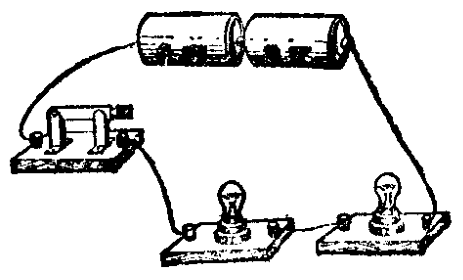
\includegraphics[width=5cm]{../pic/czwl2-ch7-27}
    \caption{}\label{fig:7-27}
    \end{minipage}
    \qquad
    \begin{minipage}{11cm}
    \centering
    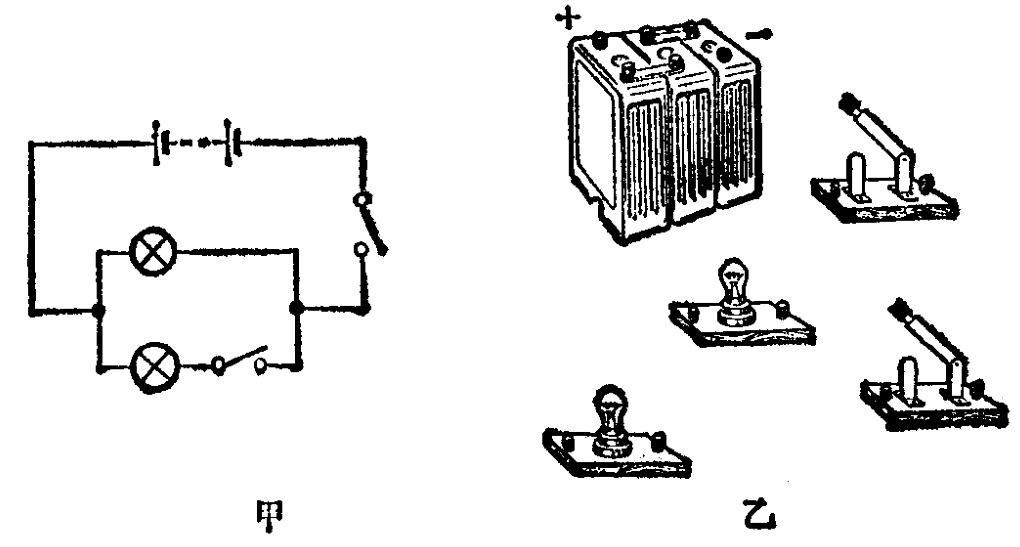
\includegraphics[width=10cm]{../pic/czwl2-ch7-28}
    \caption{}\label{fig:7-28}
    \end{minipage}
\end{figure}

(3) 按照图 \ref{fig:7-28} 甲的电路图,将图乙中的元件连成电路(元件位置不动,用铅笔线代替连接用的导线)。

(4) 有三盏电灯,想把它们连接在一个电路里,并且开关每盏电灯时不影响别的灯,应该怎样连接?画一个电路图表示出来。

(5) 在图 \ref{fig:7-29} 所示的电路中:

\begin{figure}[htbp]
    \centering
    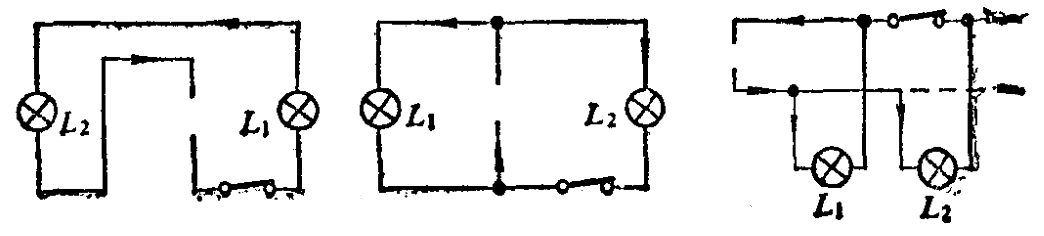
\includegraphics[width=0.7\textwidth]{../pic/czwl2-ch7-29}
    \caption{}\label{fig:7-29}
\end{figure}

\tc{1} 根据标出的电流方向,把电池组填进电路;

\tc{2} 电灯 $L_1$ 和 $L_2$ 是怎样连接的?把并联电路的干路部分用色笔描一下;

\tc{3} 如果把电键断开,各灯还能发光吗?



\section*{小实验}

\begin{figure}[htbp]
    \centering
    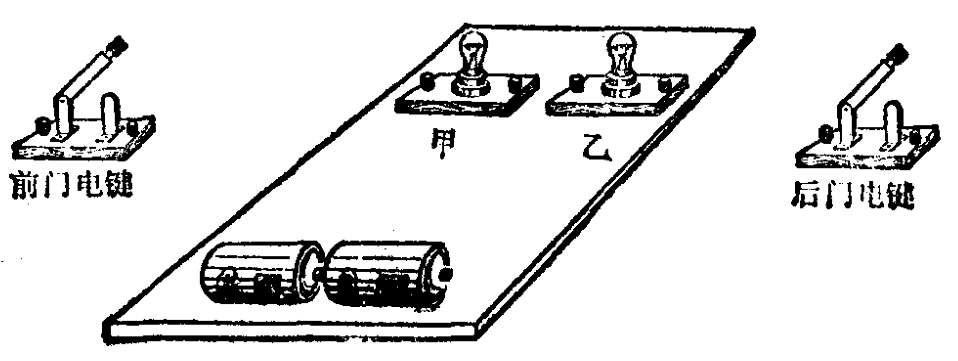
\includegraphics[width=0.7\textwidth]{../pic/czwl2-ch7-30}
    \caption{}\label{fig:7-30}
\end{figure}

图 \ref{fig:7-30} 中的木板上装着甲、乙两个小电灯和一个电池组。
假定这块木板安装在学校传达室里,学校传达室的值班人员,想从甲灯亮或乙灯亮,
知道是前门来人闭合前门电键,还是后门来人闭合后门电键。
要求这两个灯共用一个电池组。
请你替值班人员设计出符合他需要的电路,画出电路图,
再按照电路图把图 \ref{fig:7-30} 中的实物连接起来,并试验一下这个电路是否符合需要。


\section*{复习题}

(1) 怎样用实验来检查摩擦过的物体带不带电?你能提出几种办法?

(2) 人们是怎样知道电荷只有两种的?同种电荷怎样相互作用?异种电荷怎样相互作用?

(3) 试述原子的结构,并且用来解释摩擦起电现象。

(4) 什么叫导体?什么叫绝缘体?各举几个实例。
用什么样的实验可以判定一个物体是导体还是绝缘体?

(5) 电流是怎样形成的?电流的方向是如何规定的?电流有哪些效应?

(6) 什么叫电源?生活中和实验室里常用什么电源?

(7) 什么叫电路?什么叫电路图?在电路中得到持续电流的条件是什么?

(8) 什么叫串联?什么叫并联?说说你已经知道的这两种电路的区别。


